% LTeX: language=en-GB
%Author(s), Course variables
\newcommand{\titl}{02132 Assignment 2 report}
\newcommand{\subtitl}{Hardware implementation in Chisel\\of a small CPU running the image erosion}
\newcommand{\authone}{Mikkel Arn Andersen}
\newcommand{\SIDone}{s224187}
\newcommand{\authtwo}{Niclas Juul Schæffer}
\newcommand{\SIDtwo}{s224744}
\newcommand{\auththree}{Rasmus Kronborg Finnemann Wiuff}
\newcommand{\SIDthree}{s163977}
\newcommand{\lb}{\\}
%Basics
\documentclass[a4paper, english]{article}
\usepackage[utf8]{inputenc}
\usepackage[T1]{fontenc}
\usepackage[bitstream-charter]{mathdesign}
\usepackage{babel}
\usepackage[moderate, mathspacing=normal]{savetrees}
%Symbols and scientifics
\usepackage{bm}
\usepackage{physics}
\usepackage{mathtools}
\numberwithin{equation}{section}
\usepackage{siunitx}
\sisetup{
per-mode = power ,
round-mode = figures ,
round-precision = 3 ,
exponent-mode = input ,
output-decimal-marker = {.} ,
exponent-product = 	imes ,
uncertainty-mode = separate ,
range-phrase = - ,
range-units =  single ,
inter-unit-product = \ensuremath{{\cdot{}}} ,
quantity-product = \ ,
separate-uncertainty-units = single ,
}

%Appendix, TOC and Bibliography
\usepackage{appendix}
\renewcommand\appendixtocname{Appendix}
\usepackage[nottoc]{tocbibind}
\setcounter{tocdepth}{2}
\usepackage{lastpage}

%Figures
\usepackage[svgnames]{xcolor} % Required to specify font color
\usepackage{float}
\usepackage{graphicx}
\usepackage{subcaption}
\usepackage[format=plain,
    labelfont={bf,it,footnotesize},
    textfont={it,footnotesize}]{caption}
% \captionsetup[table]{name=Huskeord}
\captionsetup{font={stretch=0.9}}
\usepackage{wrapfig}
\usepackage[a4paper, centering, rmargin=2.5cm, tmargin=2.5cm, lmargin=2.5cm, bmargin=3.5cm]{geometry}
\usepackage{verbatim}
\usepackage[space]{grffile}
\usepackage[final]{pdfpages}
\usepackage{pdflscape}
\usepackage{multirow}
\usepackage{fontawesome}
\usepackage{tikz}
% \usetikzlibrary{external}
% \tikzexternalize[prefix=tikz/]
\usepackage{circuitikz}
\ctikzset{logic ports = ieee}
\usetikzlibrary{positioning}
\newcommand{\pin}[3]{\node[blue, font = \small, #2] at (#1) {#3};
                     \coordinate (#3) at (#1);}
\newcommand{\port}[4]{\node[circ, #2] (#1) {};
                     \node[#3] at (#1) {#4};}
%Header footer
\usepackage{fancyhdr}
\pagestyle{fancy}
\lhead{02132 Computer Systems \lb Assignment 1 \lb November \nth{5}}
\chead{
\includegraphics[width=.05\textwidth]{DTU}}
\rhead{\authone \ \textbf{\SIDone} \lb \authtwo \ \textbf{\SIDtwo} \lb \auththree \ \textbf{\SIDthree}}
\cfoot{Page \thepage\, of\, \pageref*{LastPage}}
\renewcommand{\headrulewidth}{0.4pt}
\renewcommand{\footrulewidth}{0.4pt}
\setlength{\headheight}{36.75034pt}

%Text tools
\usepackage{listings}
\usepackage{parcolumns}
\usepackage[super]{nth}
\usepackage[normalem]{ulem}
\usepackage{import}
\usepackage{url}
\usepackage{lipsum}
\usepackage{microtype}
\usepackage[pdfencoding=auto, psdextra]{hyperref}
\hypersetup{
    colorlinks   = true, %Colours links instead of ugly boxes
    urlcolor     = blue, %Colour for external hyperlinks
    linkcolor    = blue, %Colour of internal links
    citecolor   = red %Colour of citations
}
\usepackage[capitalise]{cleveref}
% \crefname{table}{Huskeord}{Huskeord}
\usepackage{enumitem}
\newlist{arrowlist}{itemize}{1}
\setlist[arrowlist]{label={\(\rightarrow\)}}
\usepackage{tabularray}
\UseTblrLibrary{booktabs}
\usepackage{todonotes}
\usepackage[square, longnamesfirst, numbers]{natbib}
\usepackage{empheq}
% \usepackage[newfloat, outputdir=/]{minted} % Overleaf minted buildpath fix
\usepackage[newfloat]{minted}
\setminted{fontsize=\small,
           linenos=true}
\usemintedstyle{tango}
\SetupFloatingEnvironment{listing}{listname=Listings}
\captionsetup[listing]{position=top, skip=-1pt}
\newcommand{\im}[3]{\inputminted[linenos=true, python3=true, firstline=#2, lastline=#3]{python}{#1}}
\newcommand{\java}[3]{\inputminted[linenos=true, firstline=#2, lastline=#3]{java}{#1}}
\usepackage{dirtree}

%Definitions and new commands
\newcommand{\degr}{^{\circ}}
\newcommand{\me}{\mathrm{e}}

%Title and sectioning
\def\Vhrulefill{\leavevmode\leaders\hrule height 0.7ex depth \dimexpr0.4pt-0.7ex\hfill\kern0pt}
\usepackage{titlesec}
\usepackage{titling}
\definecolor{DTUred}{cmyk}{0, .91, .72, .23}
\definecolor{FMNgrey}{cmyk}{.73,.43,.53,.38}
%Use letters insted of numbers in section numbering
% \renewcommand{\thesection}{\Alph{section}}
% \renewcommand{\thesubsection}{\Alph{subsection}}

\makeatletter
\newcommand{\github}[1]{%
   \href{#1}{\color{DTUred}\faGithub}%
}
\makeatother

%Algorithms and pseudocode
\newcounter{nalg}[section] % defines algorithm counter for chapter-level
\renewcommand{\thenalg}{\thesection .\arabic{nalg}} %defines appearance of the algorithm counter
\DeclareCaptionLabelFormat{algocaption}{Algoritme \thenalg} % defines a new caption label as Algorithm x.y

\lstnewenvironment{algorithm}[1][] %defines the algorithm listing environment
{
    \refstepcounter{nalg} %increments algorithm number
    \captionsetup{labelformat=algocaption,labelsep=colon} %defines the caption setup for: it ises label format as the declared caption label above and makes label and caption text to be separated by a ':'
    \lstset{ %this is the stype
        mathescape=true,
        frame=tB,
        numbers=left,
        numberstyle=\tiny,
        basicstyle=\scriptsize,
        keywordstyle=\color{black}\bfseries\em,
        keywords={,input, output, return, datatype, function, in, if, else, foreach, for, while, begin, end, do,} %add the keywords you want, or load a language as Rubens explains in his comment above.
        numbers=left,
        xleftmargin=.04\textwidth,
        columns=fullflexible,
        escapechar=\&,
        #1 % this is to add specific settings to an usage of this environment (for instnce, the caption and referable label)
    }
}
{}
\newcommand*{\runtimeAnalysis}[3]{\hfill\makebox[#3em][l]{\(#1\)}\hspace{5em}\makebox[#3em][l]{\(#2\)}}%

\begin{document}

\titleformat{\section}[block]
{\normalfont\Large\scshape\filright\color{DTUred}}{\fbox{\thesection}}{1em}{}

\titleformat{\subsection}
{\titlerule
    \vspace{.8ex}%
    \normalfont\scshape\color{FMNgrey}}
{\thesubsection.}{.5em}{}

\titleformat{\subsubsection}[wrap]
{\normalfont\fontseries{b}\selectfont\filright}
{\thesubsubsection.}{.5em}{}
\titlespacing{\subsubsection}
{12pc}{1.5ex plus .1ex minus .2ex}{1pc}

\title{\vspace{-40mm}\Huge\scshape\color{DTUred} \titl\lb\vspace{-4mm}\rule{4cm}{0.5mm}\lb\Large{\subtitl}}
\date{November \nth{5}}
\preauthor{\begin{center}
        \large \lineskip 0.5em%
        \begin{tabular}[t]{r}}
            \author{\textbf{Group: 22} \lb \lb \authone \ \textbf{\SIDone} \lb \authtwo \ \textbf{\SIDtwo} \lb \auththree \ \textbf{\SIDthree} \lb \href{https://github.com/rwiuff/02132Assignment2}{\color{DTUred}github.com/rwiuff/02132Assignment2} \github{https://github.com/rwiuff/02132Assignment2}}
            \postauthor{\end{tabular}\par\end{center}}
\maketitle

\pagenumbering{arabic}

\thispagestyle{empty}

\section{Work distribution}
\cref{tbl:ansvar} shows the work distribution in the group for this project.
\begin{table}[H]
    \centering
    \caption{Work distribution on the project}\label{tbl:ansvar}
    \begin{tabular}{lll}
        \toprule
        Name                 & Development tasks & Report tasks   \\
        \midrule
        Mikkel Arn Andersen  &                   &                \\
        Niclas Juul Schæffer &                   &                \\
        Rasmus Wiuff         & ISA               & \cref{sec:isa} \\
        \bottomrule
    \end{tabular}
\end{table}
\section{Design}
% \emph{Explain here what the design process was. List and describe your ISA and how the instructions are encoded. List and describe your compiled program (put a reference to attached file if the compiled program is too long to fit here). Show and describe the block diagram of your CPU. Motivate the design decision you made.}
\subsection{ISA and encoding}\label{sec:isa}
The ISA instructions are inspired from Appendix A in the assignment description. It is listed in \cref{tbl:ISA}.
\begin{table}[H]
    \centering
    \caption{Instruction-set architecture used in the assignment}\label{tbl:ISA}
    \begin{tabular}{lll}
        \toprule
        \textbf{Instruction}  & \textbf{Syntax}          & \textbf{Meaning}                  \\
        \midrule
        \multicolumn{3}{c}{Arithmetic instructions}                                          \\
        \midrule
        Addition              & \texttt{ADD Rx, Ry, Rz;} & \texttt{Rx = Ry + Rz}             \\
        Subtraction           & \texttt{SUB Rx, Ry, Rz;} & \texttt{Rx = Ry - Rz}             \\
        Immediate addition    & \texttt{ADDI Rx, Ry, z;} & \texttt{Rx = Ry + z}              \\
        Immediate subtraction & \texttt{SUBI Rx, Ry, z;} & \texttt{Rx = Ry - z}              \\
        % Multiplication        & \texttt{MUL Rx, Ry, Rz;} & \texttt{Rx = Ry \(\cdot\) Rz}     \\
        \midrule
        \multicolumn{3}{c}{Logic instructions}                                               \\
        \midrule
        Bitwise OR            & \texttt{OR Rx, Ry, Rz;}  & \texttt{Rx = Ry \(\vert\) Rz}     \\
        Bitwise AND           & \texttt{AND Rx, Ry, Rz;} & \texttt{Rx = Ry \(\&\) Rz}        \\
        Bitwise NOT           & \texttt{NOT Rx, Ry;}     & \texttt{Rx = \(\sim\)Ry}          \\
        \midrule
        \multicolumn{3}{c}{Memory instructions}                                              \\
        \midrule
        Load immediate        & \texttt{LI Rx, y;}       & \texttt{Rx = y}                   \\
        Load data             & \texttt{LD Rx, Ry;}      & \texttt{Rx = memory(Ry)}          \\
        Store data            & \texttt{SD Rx, Ry;}      & \texttt{memory(Ry) = Rx}          \\
        \midrule
        \multicolumn{3}{c}{Control and flow instructions}                                    \\
        \midrule
        Jump                  & \texttt{JMP x}           & \texttt{GOTO INST x}              \\
        Jump if equal         & \texttt{JEQ Rx, Ry, z;}  & \texttt{if(Rx == Ry) GOTO INST z} \\
        Jump if less than     & \texttt{JLT Rx, Ry, z;}  & \texttt{if(Rx < Ry) GOTO INST z}  \\
        Jump if greater than  & \texttt{JGT Rx, Ry, z;}  & \texttt{if(Rx > Ry) GOTO INST z}  \\
        % Jump if zero          & \texttt{JZ Rx, y;}       & \texttt{if(Rx == 0) GOTO INST y}  \\
        Do nothing            & \texttt{NOP;}            & \texttt{No operation}             \\
        END                   & \texttt{END;}            & \texttt{Terminate}                \\
        \bottomrule
    \end{tabular}
\end{table}
To design the instructions, first the bit sizes are considered. Some are given in the assignment. If there are 16 registers, these can be reached with \(\log_2{16} = 4\) bits. Values for the logic and arithmetic operations are 16 bit as well as addresses in the memory. The opcodes fit within 4 bits.\newline
The instruction layout is laid out in \cref{fig:inst}.
\begin{figure}[H]
    \centering
    \centering
    \caption{Instruction layout. R1 and 2 are operands, Rd is the destination register. Remaining bits are used for either memory address or immediate value.}\label{fig:inst}
    \resizebox{\textwidth}{!}{%
        \begin{tikzpicture}
            \draw[black, very thick] (0,0) rectangle (32,2); % INST box
            \draw[fill=green!20] (0,0) rectangle (4,2); % OPCODE section
            \draw[fill=red!20] (4,0) rectangle (8,2); % Reg section
            \draw[fill=blue!20] (8,0) rectangle (12,2); % Reg section
            \draw[fill=yellow!20] (12,0) rectangle (16,2); % Reg section
            \draw[fill=cyan!20] (16,0) rectangle (32,2); % Value section
            \node[align=center] (opcode) at (2,1) {\Large OPCODE (4 bits) \\ \Large 31\(\cdots\)28};
            \node[align=center] (rd) at (6,1) {\Large Rd (4 bits) \\ \Large 27\(\cdots\)24};
            \node[align=center] (r1) at (10,1) {\Large R1 (4 bits) \\ \Large 23\(\cdots\)20};
            \node[align=center] (r2) at (14,1) {\Large R2 (4 bits) \\ \Large 19\(\cdots\)16};
            \node[align=center] (val) at (24,1) {\Large Value/address (16 bit) \\ \Large 15\(\cdots\)0};
            % \node (zero) at (32,3) {\Large 0};
            % \node (thirtytwo) at (0,3) {\Large 31};
            % \draw[->, very thick] (zero) -- (32,2);
            % \draw[->, very thick] (thirtytwo) -- (0,2);
        \end{tikzpicture}
    }%
\end{figure}
\subsubsection{Opcodes}
As seen in \cref{fig:inst} there are 4 bits allocated to opcodes. \cref{tbl:ISA} accounts for seven register type operations, four jump types, three immediate types and two runtime operations.
\begin{table}[H]
    \centering
    \caption{OPCODE instruction bits.}\label{tbl:opcode}
    \begin{tabular}{lll}
        \toprule
        Instruction type           & OPCODE bits & Instruction   \\
        \midrule
        \multirow{7}{*}{Register}  & 0001        & \texttt{ADD}  \\
                                   & 0010        & \texttt{SUB}  \\
                                   & 0011        & \texttt{OR}   \\
                                   & 0100        & \texttt{AND}  \\
                                   & 0101        & \texttt{NOT}  \\
                                   & 0110        & \texttt{LD}   \\
                                   & 0111        & \texttt{SD}   \\
        \midrule
        \multirow{4}{*}{Jump}      & 1000        & \texttt{JMP}  \\
                                   & 1001        & \texttt{JEQ}  \\
                                   & 1010        & \texttt{JLT}  \\
                                   & 1011        & \texttt{JGT}  \\
        \midrule
        \multirow{3}{*}{Immediate} & 1100        & \texttt{ADDI} \\
                                   & 1101        & \texttt{SUBI} \\
                                   & 1110        & \texttt{LI}   \\
        \midrule
        \multirow{2}{*}{Runtime}   & 0000        & \texttt{NOP}  \\
                                   & 1111        & \texttt{END}  \\
        \bottomrule
    \end{tabular}
\end{table}
\subsection{Compile and encode}
\begin{listing}[H]
    \centering
    \caption[short]{The program compiled to assembly}\label{lst:ass}
    \begin{minted}{mips}
LOAD R1 <- 0
LOAD R2 <- 0
ADD R8 = R1 + R2
ADD R3 = R8 + 1
ADD R4 = R8 + 20
ADD R5 = R8 + 22
ADD R6 = R8 + 41
LOAD R3 R3
LOAD R4 R4
LOAD R5 R5
LOAD R6 R6
ADD R3 = R3 + R4
ADD R3 = R3 + R5
ADD R3 = R3 + R6
ADD R7 = R8 + 21
STORE R7 <- 255
JEQ R3 === 1020 -> 19
STORE R7 <- 000
ADD R1 = R1 + 1
JEQ R1 === 19 -> 22
JUMP -> 3
ADD R1 = 0 + 0
ADD R2 = R2 + 20
JEQ R2 === 380 -> 26
JUMP -> 3
END;
    \end{minted}
\end{listing}
\begin{landscape}
    \subsection{CPU block}
    \tikzset{ALU/.style={muxdemux, muxdemux def={
                        Lh=7, NL=2, Rh=3, NR=2, NB=0, NT=1, w=4, inset w=1, inset Lh=1, inset Rh=0, square pins=1}}}
    \tikzset{PC/.style={muxdemux, muxdemux def={
                        Lh = 6, Rh = 6, w = 6, NL = 4, NR = 1, NT = 0, NB = 0}}}
    \tikzset{ROM/.style={muxdemux, muxdemux def={
                        Lh = 6, Rh = 6, w = 6, NL = 0, NR = 2, NT = 0, NB = 0}}}
    \tikzset{RAM/.style={muxdemux, muxdemux def={
                        Lh = 6, Rh = 6, w = 6, NL = 3, NR = 1, NT = 0, NB = 0}}}
    \tikzset{REG/.style={muxdemux, muxdemux def={
                        Lh = 6, Rh = 6, w = 6, NL = 5, NR = 2, NT = 0, NB = 0}}}
    \tikzset{CU/.style={muxdemux, muxdemux def={
                        Lh = 6, Rh = 6, w = 6, NL = 1, NR = 6, NT = 0, NB = 2}}}
    \tikzset{MUX/.style={muxdemux, muxdemux def={
                        Lh=5, NL=2, Rh=2, NR=1, NB=0, NT=1, w=2, inset w=0, inset Lh=0, inset Rh=0, square pins=1}}}
    \begin{figure}[H]
        \centering
        \caption{Block diagram of the CPU architecture.}\label{fig:cpu}
        \resizebox{1.4\textwidth}{!}{
            \begin{circuitikz}
                % \draw [help lines,dashed] (-15,-10) grid (10,10);
                % \node [above] at (0,0) {Origo};
                % \node [circ] at (0,0) {};
                \node[REG, align=left] (reg) at (0,0) {\ttfamily Register \\ \ttfamily File};
                \pin{reg.lpin 1}{above left}{aSel}
                \pin{reg.lpin 2}{above left}{bSel}
                \pin{reg.lpin 3}{above left}{writeData}
                \pin{reg.lpin 4}{above left}{writeSel}
                \pin{reg.lpin 5}{above left}{writeEnable}
                \pin{reg.rpin 1}{above right}{a}
                \pin{reg.rpin 2}{above right}{b}
                \node[CU, above = 1 of reg, align=left] (cu) {\ttfamily Controll \\ \ttfamily Unit};
                \pin{cu.lpin 1}{above left}{opcode}
                \node[ALU, right = 8 of reg] (alu) {\ttfamily ALU};
                \pin{alu.lpin 1}{left}{operand 1}
                \pin{alu.lpin 2}{below left}{operand 2}
                \pin{alu.tpin 1}{right}{sel}
                \pin{alu.rpin 1}{above right}{result}
                \pin{alu.rpin 2}{below right}{comparison results}
                \node[ROM, left = 8 of reg, align=left] (rom) {\ttfamily Program \\ \ttfamily Memory};
                \pin{rom.rpin 1}{above right}{instructionRead}
                \pin{rom.rpin 2}{right}{address}
                \node[PC, above = 1 of rom, align=left] (pc) {\ttfamily Program \\ \ttfamily Counter};
                \pin{pc.lpin 1}{above left}{programCounterJump}
                \pin{pc.lpin 2}{above left}{jump}
                \pin{pc.lpin 3}{above left}{stop}
                \pin{pc.lpin 4}{above left}{run}
                \node[blue, font = \small, right, align=left] at (pc.rpin 1) {program\\Counter};
                \coordinate (step0) at (-6,2);
                \coordinate (step1) at (-6.5,0);
                \node at (rom.rpin 1 -| step1) [jump crossing] (y) {};
                \draw (rom.rpin 1) -- (y.west);
                \draw (y.east) -- (rom.rpin 1 -| step0);
                \draw (rom.rpin 1 -| step0) -- (step0 |- cu.lpin 1) -- (cu.lpin 1);
                \node[below left = .1 of cu.lpin 1] {instruction[31..28]};
                \draw (reg.lpin 1 -| step0) -- (reg.lpin 1);
                \draw (rom.rpin 1 -| step0) |- (reg.lpin 2 -| step0) -- (reg.lpin 2);
                \node at (-6,0) [jump crossing] (x) {};
                \draw (rom.rpin 1 -| step0) -| (x.north);
                \draw (x.south) |- (reg.lpin 4);
                \node[above] at (-4.5,1.3) {instruction[23..20]};
                \node[above] at (-4.5,.6) {instruction[19..16]};
                \node[above] at (-4.5,-.8) {instruction[27..24]};
                \node at (x -| y) [jump crossing] (z) {};
                \draw (cu.rpin 1) -| (2,6.5) -| (y.north);
                \draw (y.south) |- (z.north);
                \draw (z.south) |- (reg.lpin 5);
                \pin{cu.rpin 1}{above right}{writeRegister}
                \coordinate (step2) at (5.5,0);
                \node[MUX, right = 4 of reg.rpin 2, anchor = lpin 1] (alumux) {\ttfamily MUX};
                \pin{cu.rpin 5}{above right}{immediateOperand}
                \node at (reg.rpin 1 -| alumux.tpin 1) [jump crossing] (i) {};
                \node at (reg.rpin 1 -| step2) [jump crossing] (regacross) {};
                \coordinate (ramwrite) at (2.5,0);
                \coordinate (ramdata) at (3,0);
                \coordinate (ramaddress) at (3.5,0);
                \coordinate (memory) at (4,0);
                \node at (ramwrite |- reg.rpin 1) [jump crossing] (ramacross) {};
                \node at (ramwrite |- reg.rpin 2) [jump crossing] (rambcross) {};
                \node at (ramaddress |- reg.rpin 2) [jump crossing] (databcross) {};
                \node at (ramwrite |- alumux.lpin 2) [jump crossing] (ram1) {};
                \node at (ramdata |- alumux.lpin 2) [jump crossing] (ram2) {};
                \node at (ramaddress |- alumux.lpin 2) [jump crossing] (ram3) {};
                \node at (memory |- reg.rpin 1) [jump crossing] (mem1) {};
                \node at (memory |- reg.rpin 2) [jump crossing] (mem2) {};
                \node at (memory |- alumux.lpin 2) [jump crossing] (mem3) {};
                \draw (reg.rpin 1) -- (ramacross.west);
                \draw (ramacross.east) -- (mem1.west);
                \draw (mem1.east) -- (regacross.west);
                \draw (regacross.east) |- (i.west);
                \draw (i.east) -| (alu.lpin 1);
                \draw (cu.rpin 5) -| (i.north);
                \draw (cu.rpin 6) -| (regacross.north);
                \pin{cu.rpin 6}{above right}{immediateLoad}
                \draw (i.south) -- (alumux.tpin 1);
                \node at (reg.rpin 2 -| step2) [jump crossing] (j) {};
                \draw (reg.rpin 2) -- (rambcross.west);
                \draw (rambcross.east) -- (databcross.west);
                \draw (databcross.east) -- (mem2.west);
                \draw (mem2.east) -- (j.west);
                \draw (j.east) -- (alumux.lpin 1);
                \draw (alumux.rpin 1) |- (alu.lpin 2);
                \pin{alumux.lpin 1}{below}{0}
                \pin{alumux.lpin 2}{above}{1}
                \draw (cu.rpin 4) -| (alu.tpin 1);
                \pin{cu.rpin 4}{above right}{aluFunc}
                \pin{cu.rpin 2}{above right}{stop}
                \pin{cu.rpin 3}{above right}{jump}
                \coordinate (step4) at (-14.5,0);
                \coordinate (step5) at (-16.5,0);
                \coordinate (step6) at (-17,0);
                \node at (step4 |- pc.lpin 2) [jump crossing] (h) {};
                \node at (step4 |- pc.lpin 3) [jump crossing] (k) {};
                \node at (step4 |- pc.lpin 4) [jump crossing] (l) {};
                \node at (step5 |- pc.lpin 2) [jump crossing] (j1) {};
                \draw (h.east) -- (pc.lpin 2);
                \draw (cu.rpin 2) -| (4,7) -| (-16.5,5) |- (j1.north);
                \draw (j1.south) |- (k.west);
                \draw (k.east) -- (pc.lpin 3);
                \port{done}{left = 4 of pc.lpin 3}{left}{done}
                \port{run}{left = 4 of pc.lpin 4}{left}{run}
                \draw (done) -- (j1 |- pc.lpin 3);
                \draw (run) -- (l.west);
                \draw (l.east) -- (pc.lpin 4);
                \draw (pc.rpin 1) |- (-13.3,2) -- (-13.3,-2) -| (rom.rpin 2);
                \node at (-7,0) [jump crossing] (m) {};
                \draw (rom.rpin 1 -| m) -- (m.north);
                \node at (alumux.lpin 2 -| j) [jump crossing] (n) {};
                \draw (regacross.south) -- (j.north);
                \draw (j.south) -- (n.north);
                \draw (m.south) |- (ram1.west);
                \draw (ram1.east) -- (ram2.west);
                \draw (ram2.east) -- (ram3.west);
                \draw (ram3.east) -- (mem3.west);
                \draw (mem3.east) -- (n.west);
                \draw (n.east) -- (alumux.lpin 2);
                \node at (-4, -2) {instruction[15..0]};
                \draw (reg.lpin 3) -- (x.east);
                \draw (x.west) -- (z.east);
                \draw (z.west) -- (m.east);
                \node[MUX, below = 1 of n.south, anchor = tpin 1] (immediateMux) {\ttfamily MUX};
                \coordinate (aluOutCoord) at (13.5,0);
                \node at (alu.rpin 1 -| aluOutCoord) [jump crossing] (aluOutCross) {};
                \node at (alumux |- immediateMux.lpin 2) [jump crossing] (immediateMuxCross) {};
                \draw (alu.rpin 1) -- (aluOutCross.west);
                \draw (aluOutCross.east) -- ++(1.2,0) |- (immediateMuxCross.east);
                \draw (immediateMuxCross.west) -| (6.5,-6.7) -| (immediateMux.lpin 2);
                \draw (n.south) -- (immediateMux.tpin 1);
                \draw (n -| immediateMux.lpin 1) |- (immediateMux.lpin 1);
                \pin{immediateMux.lpin 1}{below}{1}
                \pin{immediateMux.lpin 2}{above}{0}
                \draw (immediateMux.rpin 1) -| (immediateMuxCross.north);
                \draw (pc.lpin 1) -| (h.north);
                \draw (h.south) -- (k.north);
                \draw (k.south) -- (l.north);
                \draw (l.south) |- (-8, -2.5);
                \coordinate (jumpcoord) at (-8,0);
                \draw (rom.rpin 1 -| jumpcoord) -- (-8, -2.5);
                \node[above] at (-10.2,-3) {instruction[15..0]};
                \node [or port, right = 4 of cu.rpin 2, anchor = in 2] (or) {\ttfamily OR};
                \draw (alu.rpin 2) -| (aluOutCross.south);
                \draw (aluOutCross.north) |- (or.in 2 |- cu.rpin 3) -| (or.in 2);
                \draw (cu.rpin 3) -| (5.5,5) |- (or.in 1);
                \draw (or.out) |- (5,8) -| (-17.5,5.5) |- (j1.west);
                \draw (j1.east) -- (h.west);
                \pin{cu.bpin 1}{left}{writeToMemory}
                \draw (cu.bpin 1) |- (2,2);
                \draw (2,2) -| (ramacross.north);
                \draw (ramacross.south) -- (rambcross.north);
                \draw (rambcross.south) -- (ram1.north);
                \draw (reg.rpin 1 -| ramaddress) -- (databcross.north);
                \draw (databcross.south) -- (ram3.north);
                \draw (reg.rpin 2 -| ramdata) -- (ram2.north);
                \node[RAM, below = 2.5 of reg, align=left] (ram) {\ttfamily Data \\ \ttfamily Memory};
                \pin{ram.lpin 1}{above left}{dataWrite}
                \pin{ram.lpin 2}{above left}{address}
                \pin{ram.lpin 3}{above left}{writeEnable}
                \pin{ram.rpin 1}{above right}{dataRead}
                \draw (ram1.south) |- (-4.5,-2.5) |- (ram.lpin 3);
                \draw (ram2.south) |- (-4,-3) |- (ram.lpin 2);
                \draw (ram3.south) |- (-3.5,-3.5) |- (ram.lpin 1);
                \pin{cu.bpin 2}{below}{loadFromMemory}
                \draw (cu.bpin 2) -| (mem1.north);
                \draw (mem1.south) -- (mem2.north);
                \draw (mem2.south) -- (mem3.north);
                \node at (-7.5,-4.5) [jump crossing] (writeX) {};
                \node[MUX, left = 1 of writeX, anchor = tpin 1] (writeMux) {\ttfamily MUX};
                \node at (-7, -8) [jump crossing] (writeMuxX) {};
                \draw (ram.rpin 1) |- (-6,-8) -| (writeMuxX.east);
                \draw (writeMuxX.west) -| (writeMux.lpin 2);
                \draw (mem3.south) |- (-6,-8.5) -| (writeMuxX.south);
                \draw (writeMuxX.north) |- (writeX.east);
                \draw (writeX.west) -- (writeMux.tpin 1);
                \draw (immediateMuxCross.south) |- (-10,-9) |- (writeMux.lpin 1);
                \draw (writeMux.rpin 1) -| (writeX.south);
                \draw (writeX.north) |- (m.west);
                \pin{writeMux.lpin 1}{below}{0}
                \pin{writeMux.lpin 2}{above}{1}
            \end{circuitikz}
        }
    \end{figure}
\end{landscape}
\section{Implementation}
\emph{Briefly discuss the implementation in Chisel of your design. You can include some code snippets if these are relevant to explain certain aspects of the implementation. In other words, try to answer the question “What does a reader need to know about your Chisel implementation?”}
\section{Test and analysis}
\emph{Report here the results from the test you have carried out. Present the test you have developed (if any). Remember to discuss the results and the test you have carried out, do not just present them, but explain and argue their meaning. Address the design evaluation questions listed in Task 11 in the Assignment 2 document.}
% \section{References}
\begin{thebibliography}{1}
    \bibitem{arduino}
    Arduino, José Bagur, Taddy Chung \emph{Arduino Memory Guide (19/09/2023)\newline \href{https://docs.arduino.cc/learn/programming/memory-guide}{https://docs.arduino.cc/learn/programming/memory-guide}}
\end{thebibliography}
%Bibliography herunder:
%\newpage

%\bibliographystyle{unsrtnat}
%\bibliography{Bibliography}

%\newpage

%\listoffigures
% \newpage
% \listoftables
%\newpage

%Appendicer herunder:

%\input{Appendix.tex}

\end{document}